% Compile twice!
% With the current MiKTeX, you need to install the beamer, and the translator packages directly form the package manager!

\documentclass{beamer}
\usepackage{tikz}
\usetikzlibrary{shapes,arrows}

\usepackage[T1]{fontenc}
\usepackage{amsfonts}
\usepackage{amsmath}
\usepackage[utf8]{inputenc}

\usetheme{boxes}

% tikz settings for the flowchart(s)

% Define block styles

\tikzstyle{decision} = [diamond, minimum width=3cm, minimum height=1cm, text centered, draw=black, fill=green!15]
\tikzstyle{block} = [rectangle, draw, fill=blue!15, text width=20em, text centered, minimum height=1em]
    
\tikzstyle{line} = [draw, -latex']
\tikzstyle{cloud} = [draw, ellipse,fill=red!20, node distance=3cm,
    minimum height=2em]
\tikzstyle{arrow} = [thick,->,>=stealth]

\begin{document}

\begin{frame}[plain]
\begin{tikzpicture}[overlay, remember picture]
\node[anchor=center] at (current page.center) {
\begin{beamercolorbox}[center]{title}
    {\Huge A Számítástudomány Alapjai I}\\
    {\Large Vizsgatételek}
\end{beamercolorbox}};
\end{tikzpicture}
\end{frame}

% --------------------  LOGIKA --------------------

\begin{frame}[plain]
\begin{tikzpicture}[overlay, remember picture]
\node[anchor=center] at (current page.center) {
\begin{beamercolorbox}[center]{title}
    {\Huge Logika}
\end{beamercolorbox}};
\end{tikzpicture}
\end{frame}


\begin{frame}

\begin{block}{Tétel: Minden formula egyértelműen olvasható}
F formulára a következő állítások közül pontosan egy teljesül:

\begin{enumerate}
\item F egy változó.
\item Pontosan egy G formulára $F = \neg G$
\item Pontosan egy G és pontosan egy H formuláta $F = (G \land H)$
\item Pontosan egy G és pontosan egy H formulára $F = (G \lor H)$
\end{enumerate}

\end{block}

\end{frame}


\begin{frame}

\begin{block}{Tétel: Az ítéletkalkulus kompaktsági tétele}
Egy formulahalmaz akkor és csak akkor elégíthető ki, ha minden véges részhalmaza kielégíthető.

\end{block}

\begin{block}{Tétel: Adekvát halmazok}
$\{\neg, \lor, \land\}, \{\neg, \lor\}, \{\neg, \land\}$ adekvát (azaz bármilyen formula leírható ezekkel), $\{\lor, \land\}$ nem adekvát.

\end{block}

\end{frame}


\begin{frame}

\begin{block}{tétel: Equivalens állítások formulákra}
Legyenek $F, F_1, ... , F_n$ tetszőleges formulák, ekkor a következő állítások equivalensek:

\begin{enumerate}
\item $\{F_1, ... , F_n\} \models F$
\item $F_1 \land ... \land F_n \implies F$ tautológia
\item $F_1 \land ... \land F_n \land \neg F$ kielégíthetetlen.
\end{enumerate}

\end{block}

\end{frame}

\begin{frame}

\begin{block}{Lemma: Helyettesítési Lemma}
Legyenek $F, G, H$ formulák úgy, hogy $F \equiv G$ és $F$ a $G$ részformulája.\\
Ha $H[F/G]$ azt a formulát jelöli, amelyben $F$ valamely előfordulását helyettesítettük $G$-vel, akkor
$$H \equiv H[F/G]$$

\end{block}

\end{frame}


\begin{frame}

\begin{block}{Tétel: Konjunktív és diszjunktív normálforma létezése}
Minden $F$ Formulához létezik vele logikailag ekvivalens konjunktív és diszjunktív normálforma.

\end{block}

\begin{block}{Bizonyítás}
Konjunktív:
\begin{enumerate}
	\item (Negáció bevitele.) Amíg lehetséges, helyettesítsük $F$-ben a
	\begin{itemize}
		\item $\neg \neg G$ alakú részformulákat $G$-vel,
		\item $\neg (G \land H)$ alakú részformulákat $\neg G \lor \neg H$-val,
		\item $\neg (G \lor H)$ alakú részformulákat $\neg G \land \neg H$-val.
	\end{itemize}
	\item Amíg lehetséges, helyettesítsük $F$-ben a
	\begin{itemize}
		\item $F \lor (G \land H)$ alakú részformulákat $(F \lor G) \land (F \lor H)$-val,
		\item $(F \land G) \lor H$ alakú részformulákat $(F \lor H) \land (G \lor H)$-val.
	\end{itemize}
\end{enumerate}

Diszjunktív:
\begin{enumerate}
	\item Ugyanaz mint a konjunktív normálforma esetén.
	\item Amíg lehetséges, helyettesítsük $F$-ben a
	\begin{itemize}
		\item $F \land (G \lor H)$ alakú részformulákat $(F \land G) \lor (F \land H)$-val,
		\item $(F \lor G) \land H$ alakú részformulákat $(F \land H) \lor (G \land H)$-val.
	\end{itemize}
\end{enumerate}
\end{block}

\end{frame}

\begin{frame}

\begin{block}{Tétel: Dedukció tétel}
Tetszőleges $\Sigma$ formulahalmaz esetén $\Sigma \vdash F \rightarrow G$ akkor és csak akkor teljesül, ha $\Sigma \cup \{F\} \vdash G$.

\end{block}

\begin{block}{Tétel: Dichotómia tétel}
Tetszőleges $\Sigma$ formulahalmaz esetén, ha $\Sigma \cup \{F\} \vdash$ (levezethető) $G$ és $\Sigma \cup \{\neg F\} \vdash G$, akkor $\Sigma \vdash G$.\\
("Az $F$ Formula nem szól bele").

\end{block}

\begin{block}{Tétel: Helyességi tétel}
Tetszőleges $\Sigma$ és $F$ esetén, ha $\Sigma \vdash F$, akkor $\Sigma \models F$.\\
(Helyes, ha csak az elélethez tartozó formulákat lehet bizonyítani.)

\end{block}

\begin{block}{Tétel: Teljességi tétel}
Minden $\Sigma$-ra és $F$-re, ha $\Sigma \models F$, akkor $\Sigma \vdash F$.\\
(Teljes, ha minden, az elmélethez tartozó formulát be lehet bizonyítani.)

\end{block}

\begin{block}{Tétel: Konzisztencia tétel}
Tetszőleges formulahalmaz, akkor és csak akkor konzisztens, ha kielégíthető.\\
(Konzisztens, ha nem vezethető le belőle a $\downarrow$.)

\end{block}

\end{frame}

% --------------------  GRÁFELMÉLET --------------------

\begin{frame}[plain]
\begin{tikzpicture}[overlay, remember picture]
\node[anchor=center] at (current page.center) {
\begin{beamercolorbox}[center]{title}
    {\Huge Gráfelmélet}
\end{beamercolorbox}};
\end{tikzpicture}
\end{frame}


\begin{frame}

\begin{block}{Tétel: Fokszám-Élszám}
Legyen $G = (V, E)$ (Gráf). Ekkor $G$-ben a páratlan fokú csúcsok száma páros.

\end{block}

\begin{block}{Bizonyítás}
$$\sum_{a \in V} d(a) = \sum_{d(a) \equiv 0 (mod 2)} d(a) + \sum_{d(a) \equiv 1 (mod 2)} \equiv 0 (mod 2)$$
amiből kapjuk, hogy $$\sum_{d(a) \equiv 1 (mod 2)} d(a) \equiv 0 (mod 2)$$.

\end{block}

\end{frame}

\begin{frame}

\begin{block}{Tétel: Equivalens állítások fákra}
Egy $G$ egyszerű gráfra a következő állítások equivalensek:

\begin{enumerate}
\item $G$ Fa
\item $G$ Összefüggő, de bármely él elhagyásával kapott részgráf már nem összefüggő.
\item Ha $v, v'$ a $G$ különböző csúcsai, akkor pontosan egy út vezet $v$-ből $v'$be.
\item $G$-ben nincs kör, de bármely új él hozzáadásával kapott gráf már tartalmaz kört.
\end{enumerate}

\end{block}


\begin{block}{Tétel: Elsőfokú pontok}
Ha egy véges gráfban nincs kör, de van él, akkor van benne legalább két elsőfokú pont.

\end{block}

\end{frame}

\begin{frame} 

\begin{block}{Tétel: Ekvivalens állítások n-pontú fákra}
Egy $G$ egyszerű gráfra a következő álítások ekvivalensek:

\begin{enumerate}
\item $G$ fa.
\item $G$-ben nincs kör és $n - 1$ éle van.
\item $G$ összefüggő és $n - 1$ éle van.
\end{enumerate}

\end{block}

\begin{block}{Tétel: Feszítőfa létezése}
Minden véges összefüggő $G$ gráfnak létezik feszítőfája.

\end{block}

\end{frame}

\begin{frame} 

\begin{block}{Tétel: Körök száma}
Egy véges összefüggő $G = (E, V)$ gráfban létezik \underline{legalább} $e(G) - v(G) + 1$ különböző kör.

\end{block}

\begin{block}{Bizonyítás}
A feszítőfa létezése téltel miatt ($\Rightarrow$) $\exists T$ feszítőfa, aminek $v(G) - 1$ éle van.\\
Legyen $K_f$ az a kör, ami $T \cup \{f\}$-ben van, ahol $f \in E(G) \setminus E(T)$\\
$T_G$ komplementerben legalább $e(G) - e(T) = e(G) - (v(G) - 1) = e(G) - v(G) - 1$ ilyen $f$ él van.\\
$\Rightarrow$ legalább $e(G) - v(G) + 1$ különbző kör.

\end{block}

\end{frame}

\begin{frame}
\begin{block}{Tétel: Vágások száma}
Egy véges összefüggő $G = (V, E)$ gráfban létezik legalább $v(G) - 1$ vágás.
\end{block}

\begin{block}{Bizonyítás}
$T$ Feszítőfa összefüggő.\\
$\Rightarrow$ $T_G$ komplementer nem vágás.\\
Ha $T_G$ komplementerhez hozzáveszünk egy élt $T$-ből, akkor elvágó élhalmazt kapunk, amely tartalmaz egy vágást.\\
Ez a vágás tartalmazza $e$ élt, de másikat nem $T$ből.\\
Mivel $T$-nek $v(G) - 1$ éle van $\Rightarrow$ legalább ennyi különböző vágást kapunk.

\end{block}

\end{frame}

\begin{frame}

\begin{block}{Tétel: Euler gráfok}
Ha $G$ összefüggő véges gráf, akkor a következő állítások ekvivalensek:\\
\begin{enumerate}
\item $G$ Euler-gráf.
\item $d(v)$ páros minden $v \in V(G)$-re.
\item $G$ éldiszjunkt körök egyesítése.
\end{enumerate}
\end{block}

\end{frame}

\begin{frame}

\begin{block}{Tétel: Ore tétel}
Legyen $G$ egy $n \geq 3$ pontú egyszerű véges gráf. Ha $$d(v) + d(w) \geq n$$ minden $v$, $w$ nem-szomszédos pontra, akkor $G$ Hamilton-gráf.

\end{block}

\begin{block}{Tétel: Dirac tétel}
Legyen $G$ egy $n \geq 3$ pontú egyszerű véges gráf. Ha $$d(v) \geq \frac{n}{2}$$ minden $v$ csúcsra, akkor $G$ Hamilton-gráf.

\end{block}

\end{frame}

\begin{frame}

\begin{block}{Tétel: Kruskal algoritmus}
Legyen $G = (V, E, fi , w)$ egy véges összefüggő gráf. A következő algoritmus megtalál egy minimális súlyú feszítőfát $G$-ben.
    
\end{block}

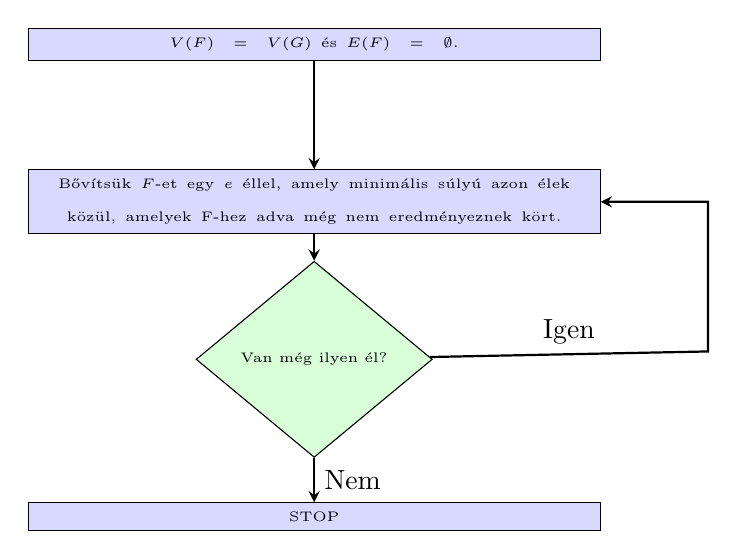
\begin{tikzpicture}[node distance = 2cm, auto]
    % Place nodes
    \node [block] (step1) {\tiny{$V(F)=V(G)$ és $E(F) = \emptyset$.}};
    \node [block, below of=step1] (step2) {\tiny{Bővítsük $F$-et egy $e$ éllel, amely minimális súlyú azon élek közül, amelyek F-hez adva még nem eredményeznek kört.}};
    \node [decision, below of=step2] (step3) {\tiny{Van még ilyen él?}};
    \node [block, below of=step3] (step4) {\tiny{STOP}};

    \draw [arrow] (step1) -- (step2);
    \draw [arrow] (step2) -- (step3);
	\draw [arrow] (step3) -- node {Nem} (step4);    
    \draw[arrow] (step3) -- node {Igen} + (5, 0.1) |- (step2);
    

\end{tikzpicture}

\end{frame}

\begin{frame}

\begin{block}{Tétel: Erős összefüggőség}

\end{block}

\end{frame}

\end{document}